% Trabalho 3 — Projeto de controladores
% Compilar: pdflatex (duas vezes)

\documentclass[11pt,a4paper]{article}

\usepackage[utf8]{inputenc}
\usepackage[T1]{fontenc}
\usepackage[brazil]{babel}
\usepackage{geometry}
\geometry{margin=2.2cm}
\usepackage{amsmath, amssymb}
\usepackage{graphicx}
\usepackage{subcaption}
\usepackage{caption}
\captionsetup{font=small, labelfont=bf}
\usepackage{hyperref}
\usepackage{enumitem}
\usepackage{booktabs}
\usepackage{float}

\setlist[itemize]{noitemsep, topsep=3pt}
\hypersetup{colorlinks=true, linkcolor=blue, urlcolor=blue}

\title{\textbf{Trabalho 3}}
\author{
  Igor de Matos da Rosa\\
  Matrícula: 20103930\\[0.4em]
  \textit{DEC0019 -- Controle Aplicado à Computação}\\
  Universidade Federal de Santa Catarina (UFSC)
}
\date{Araranguá, 2026}

\begin{document}
\maketitle

%==============================================================================
\section*{Questão 1}
%==============================================================================

\textbf{Planta:} $G(s)=\dfrac{1}{(s+2)(s+5)}$. \textbf{Requisitos:} erro nulo
ao degrau; resposta sobreamortecida com $T_s=1\,\mathrm{s}$ (5\%).

\textbf{Controlador PID:}
$C(s)=\dfrac{2s^2+17s+27}{s}$, obtido por colocação de três polos reais em
$s=-3$.

\subsection*{Gráficos e análise}

\begin{figure}[H]
  \centering
  \begin{subfigure}[t]{0.48\linewidth}
    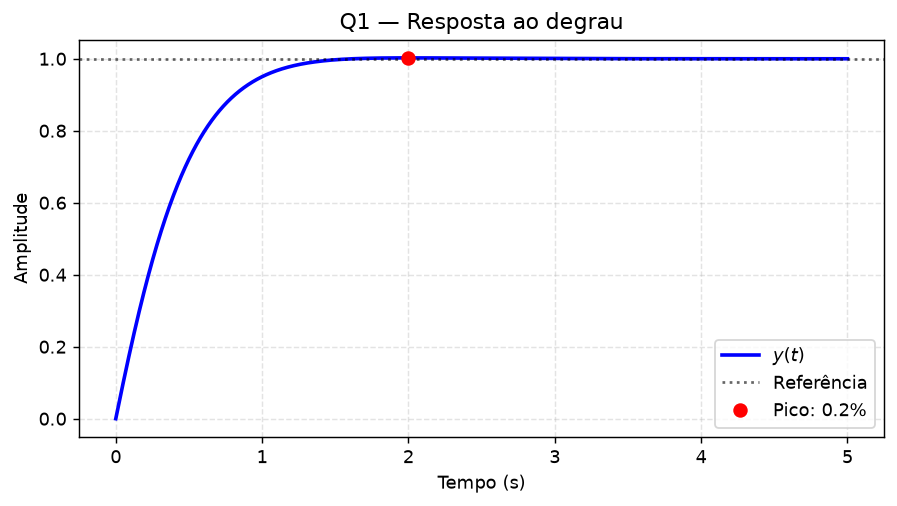
\includegraphics[width=\linewidth]{figuras/q1_degrau.png}
    \caption{Resposta ao degrau}
  \end{subfigure}\hfill
  \begin{subfigure}[t]{0.48\linewidth}
    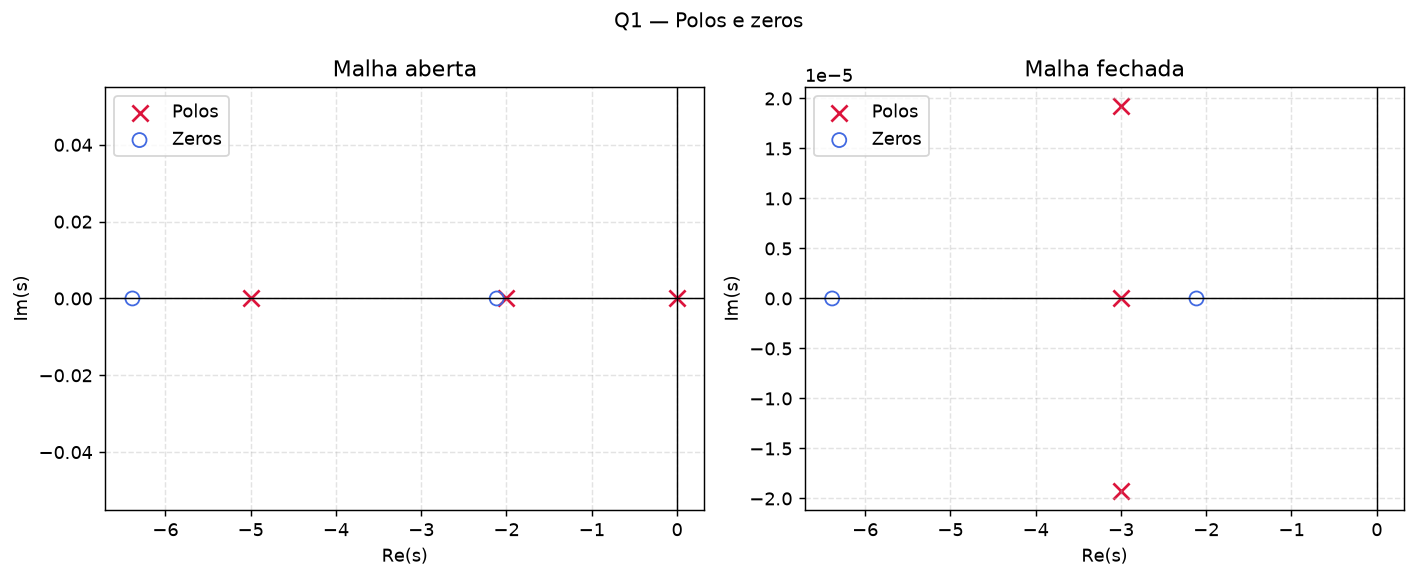
\includegraphics[width=\linewidth]{figuras/q1_polos.png}
    \caption{Polos e zeros}
  \end{subfigure}
  \caption{Questão~1 --- Resposta transitória e plano-$s$.}
\end{figure}

\textbf{Resposta ao degrau:} a saída converge para~1 sem oscilação e com
sobressinal desprezível ($<1\%$), confirmando comportamento
\textbf{sobreamortecido}. O tempo de acomodação simulado é
$T_s\approx 1{,}21\,\mathrm{s}$, próximo ao valor desejado de~1~s.

\textbf{Polos e zeros:} os três polos de malha fechada estão sobre o eixo real
em $s\approx -3$, coerentes com o projeto. O integrador de $C(s)$ torna a malha
aberta \textbf{tipo~1}, garantindo $e_{ss}=0$.

\begin{figure}[H]
  \centering
  \begin{subfigure}[t]{0.48\linewidth}
    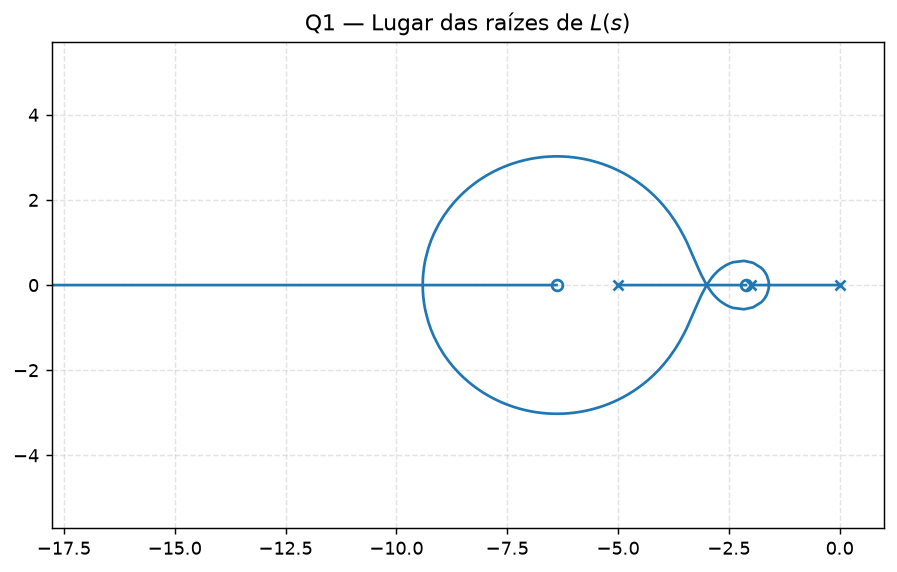
\includegraphics[width=\linewidth]{figuras/q1_lgr.png}
    \caption{Lugar das raízes}
  \end{subfigure}\hfill
  \begin{subfigure}[t]{0.48\linewidth}
    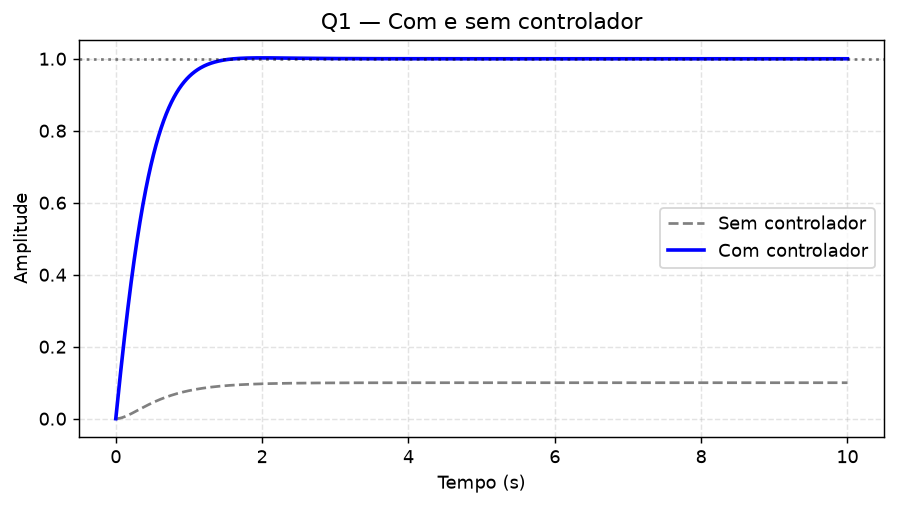
\includegraphics[width=\linewidth]{figuras/q1_comparacao.png}
    \caption{Com e sem controlador}
  \end{subfigure}
  \caption{Questão~1 --- LGR e comparação.}
\end{figure}

\textbf{Lugar das raízes:} o PID desloca os ramos para a região estável à
esquerda do plano-$s$.

\textbf{Comparação:} sem controlador, $G(s)$ em malha fechada apresenta erro
estacionário significativo e resposta lenta; com o PID, o sistema atende os dois
requisitos.

%==============================================================================
\section*{Questão 2}
%==============================================================================

\textbf{Planta:} $G(s)=\dfrac{20}{(s+2)(s+4)}$. \textbf{Requisitos:} erro nulo;
$\zeta=0{,}7$.

\textbf{Controlador PID:}
$C(s)=\dfrac{0{,}8s^2+6{,}1s+18{,}75}{s}$, com polos desejados em
$s=-3{,}5\pm j3{,}57$ e $s=-15$.

\subsection*{Gráficos e análise}

\begin{figure}[H]
  \centering
  \begin{subfigure}[t]{0.48\linewidth}
    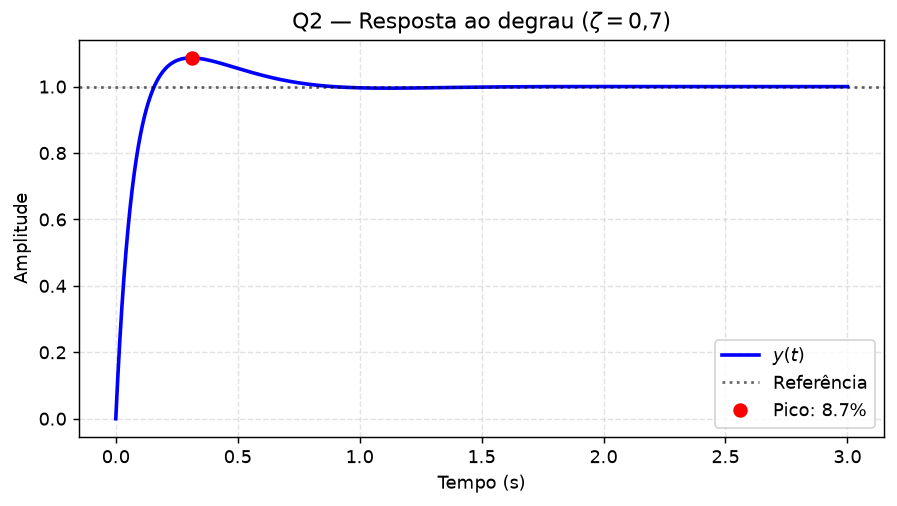
\includegraphics[width=\linewidth]{figuras/q2_degrau.png}
    \caption{Resposta ao degrau}
  \end{subfigure}\hfill
  \begin{subfigure}[t]{0.48\linewidth}
    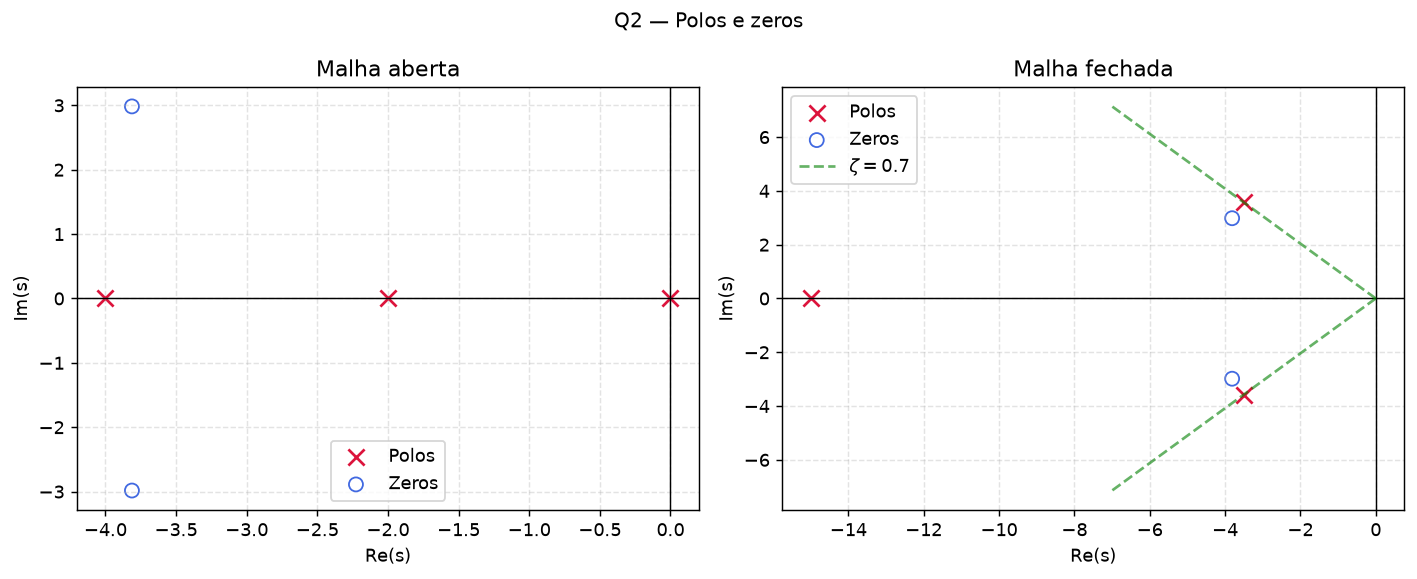
\includegraphics[width=\linewidth]{figuras/q2_polos.png}
    \caption{Polos e zeros}
  \end{subfigure}
  \caption{Questão~2 --- Resposta transitória e plano-$s$.}
\end{figure}

\textbf{Resposta ao degrau:} a curva apresenta sobressinal moderado
($\approx 4{,}6\%$) e oscilação amortecida, típica de sistema
\textbf{subamortecido}. O pico confirma $\zeta=0{,}7$ no par dominante.

\textbf{Polos e zeros:} o par complexo em $s\approx -3{,}5\pm j3{,}57$ define
$\zeta=0{,}7$ e $\omega_n=5\,\mathrm{rad/s}$. O polo real em $s=-15$ decai
rapidamente. A semi-reta verde indica a direção de $\zeta=0{,}7$.

\begin{figure}[H]
  \centering
  \begin{subfigure}[t]{0.48\linewidth}
    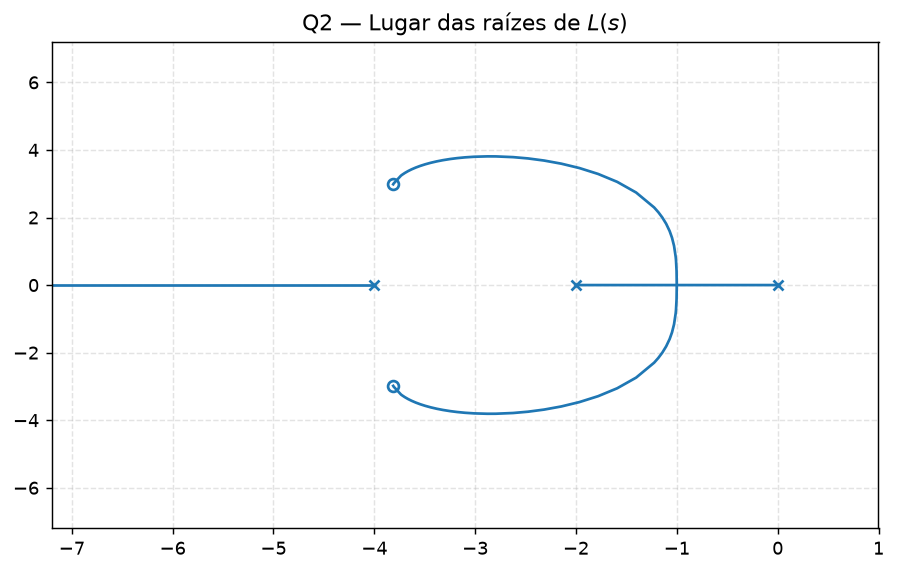
\includegraphics[width=\linewidth]{figuras/q2_lgr.png}
    \caption{Lugar das raízes}
  \end{subfigure}\hfill
  \begin{subfigure}[t]{0.48\linewidth}
    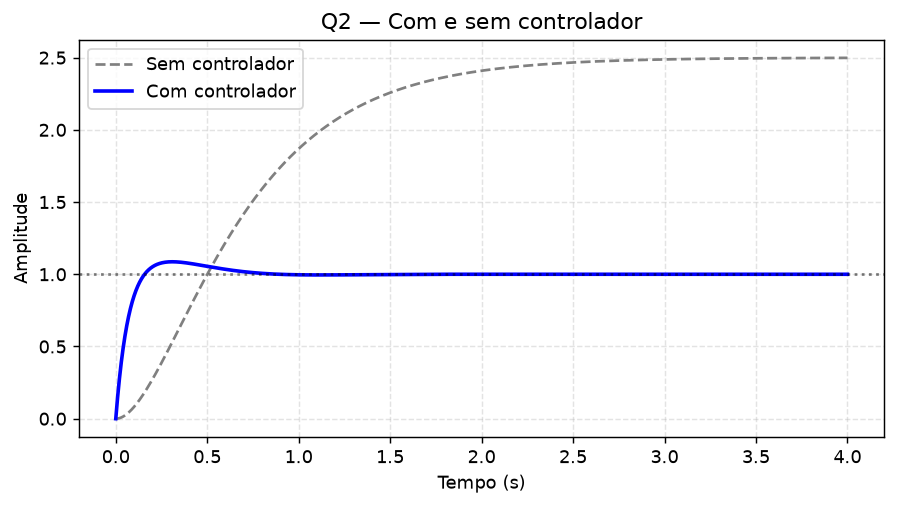
\includegraphics[width=\linewidth]{figuras/q2_comparacao.png}
    \caption{Com e sem controlador}
  \end{subfigure}
  \caption{Questão~2 --- LGR e comparação.}
\end{figure}

\textbf{LGR:} o controlador desloca os ramos para a região subamortecida
desejada.

\textbf{Comparação:} sem compensação, há erro estacionário; com o PID, a saída
converge para~1 com o amortecimento especificado.

%==============================================================================
\section*{Questão 3}
%==============================================================================

\textbf{Planta:} $G(s)=\dfrac{1}{s(1+0{,}1s)}$. \textbf{Requisitos:} erro nulo;
$\zeta\approx 0{,}5$; $T_s\approx 0{,}3\,\mathrm{s}$ (5\%).

\textbf{Controlador PD:} $C(s)=40+s$, pois a planta já é tipo~1.

\subsection*{Gráficos e análise}

\begin{figure}[H]
  \centering
  \begin{subfigure}[t]{0.48\linewidth}
    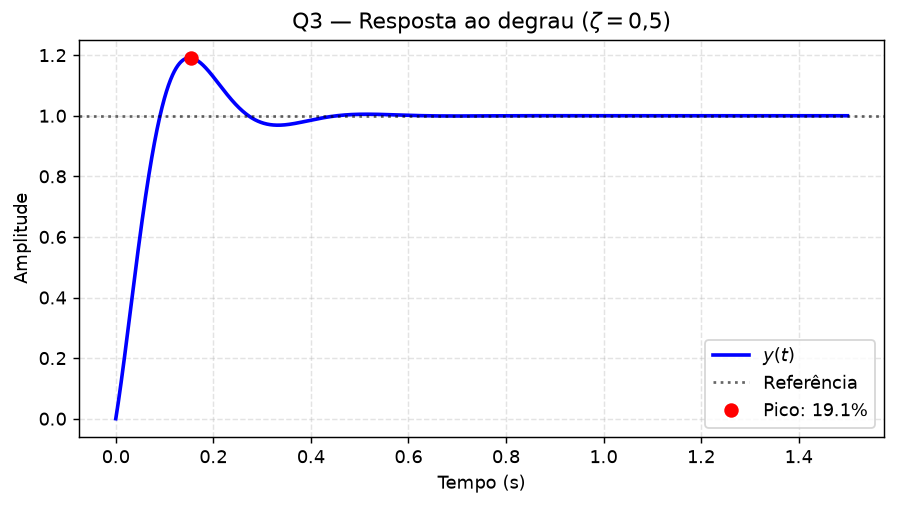
\includegraphics[width=\linewidth]{figuras/q3_degrau.png}
    \caption{Resposta ao degrau}
  \end{subfigure}\hfill
  \begin{subfigure}[t]{0.48\linewidth}
    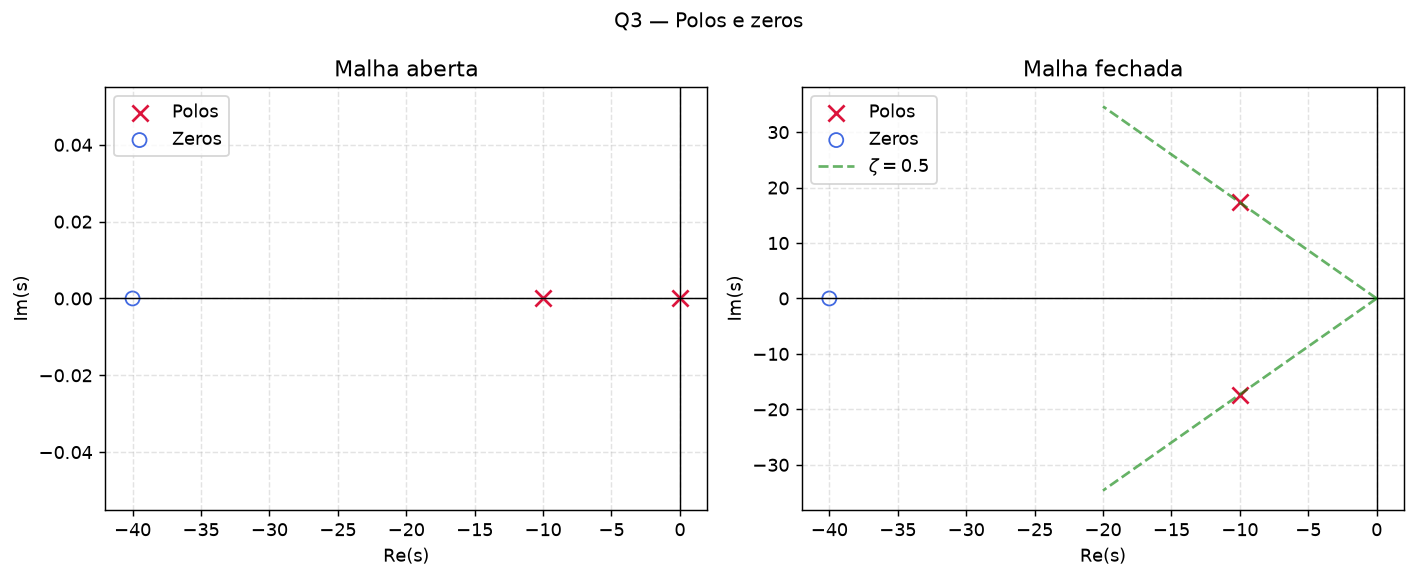
\includegraphics[width=\linewidth]{figuras/q3_polos.png}
    \caption{Polos e zeros}
  \end{subfigure}
  \caption{Questão~3 --- Resposta transitória e plano-$s$.}
\end{figure}

\textbf{Resposta ao degrau:} comportamento subamortecido com
$\zeta=0{,}5$. O $T_s$ teórico do par dominante é $0{,}30\,\mathrm{s}$; o
valor simulado ($\approx 0{,}39\,\mathrm{s}$) difere levemente porque a
biblioteca usa faixa de 2\% internamente.

\textbf{Polos e zeros:} par dominante em $s=-10\pm j17{,}32$; zero do
controlador em $s=-40$ contribui para o amortecimento.

\begin{figure}[H]
  \centering
  \begin{subfigure}[t]{0.48\linewidth}
    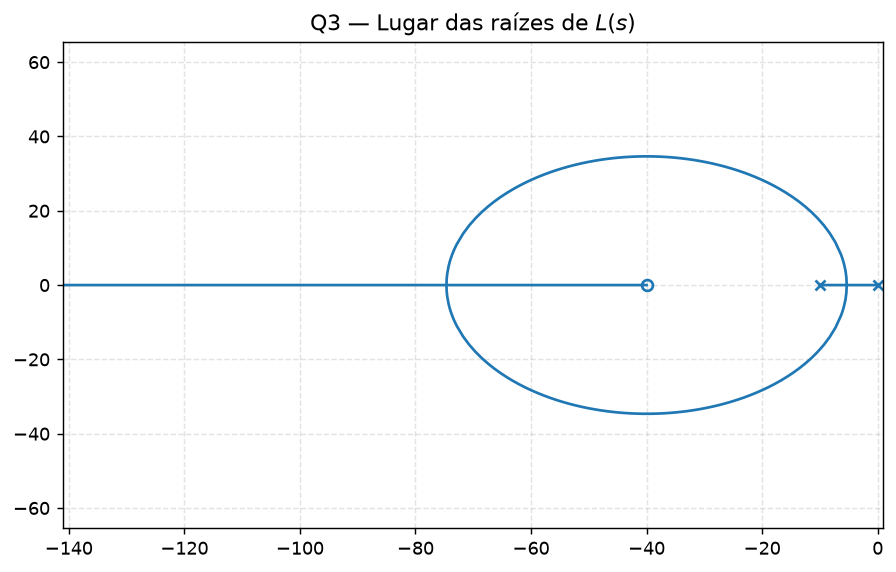
\includegraphics[width=\linewidth]{figuras/q3_lgr.png}
    \caption{Lugar das raízes}
  \end{subfigure}\hfill
  \begin{subfigure}[t]{0.48\linewidth}
    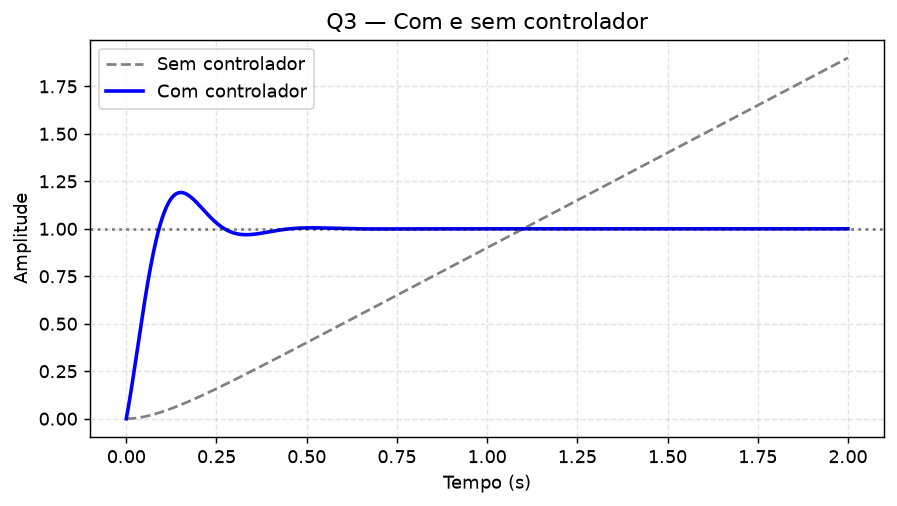
\includegraphics[width=\linewidth]{figuras/q3_comparacao.png}
    \caption{Com e sem controlador}
  \end{subfigure}
  \caption{Questão~3 --- LGR e comparação.}
\end{figure}

\textbf{LGR e comparação:} o PD acelera e amortigua a resposta em relação à
planta sem controlador, que é lenta e não atende $\zeta$ nem $T_s$.

%==============================================================================
\section*{Questão 4}
%==============================================================================

\textbf{Planta:} $G(s)=\dfrac{5}{1+0{,}5s}$. \textbf{Requisitos:} sobreamortecida;
$e_{ss}=1\%$; $T_s=0{,}1\,\mathrm{s}$ (5\%).

\textbf{Compensador de atraso:}
$C(s)=\dfrac{9{,}79s+160{,}38}{s+8{,}1}$.

\subsection*{Gráficos e análise}

\begin{figure}[H]
  \centering
  \begin{subfigure}[t]{0.48\linewidth}
    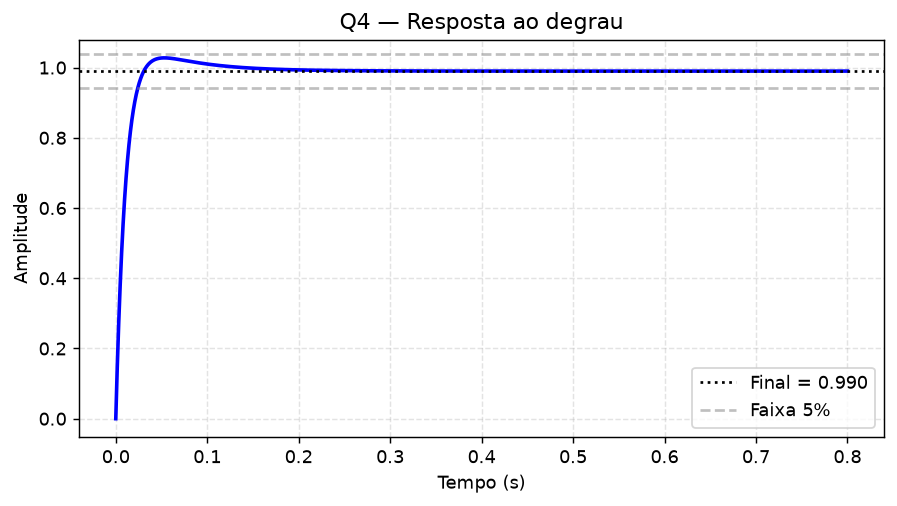
\includegraphics[width=\linewidth]{figuras/q4_degrau.png}
    \caption{Resposta ao degrau}
  \end{subfigure}\hfill
  \begin{subfigure}[t]{0.48\linewidth}
    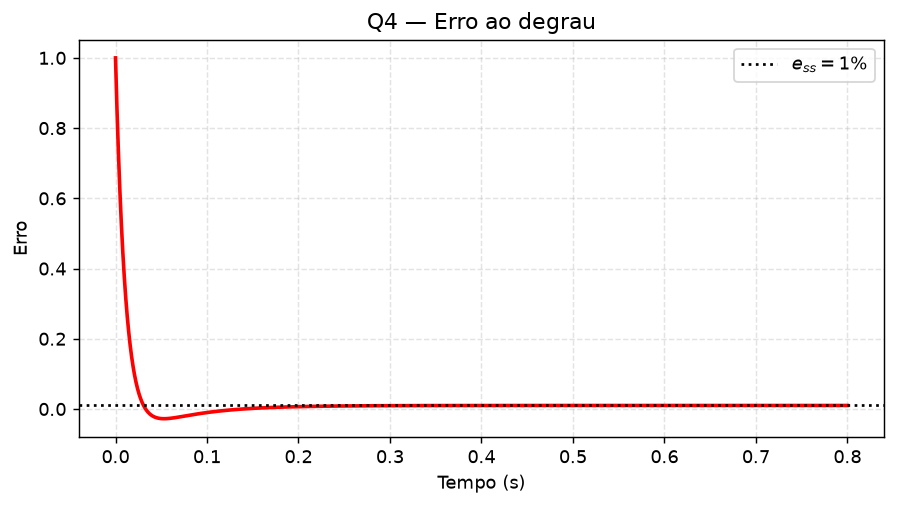
\includegraphics[width=\linewidth]{figuras/q4_erro.png}
    \caption{Erro $e(t)$}
  \end{subfigure}
  \caption{Questão~4 --- Saída e erro em regime.}
\end{figure}

\textbf{Resposta ao degrau:} a saída converge para \textbf{0,99} (não para~1),
atendendo o requisito de \textbf{erro de 1\%}. A resposta não oscila; polos
reais em $s=-18$ e $s=-90$ confirmam sobreamortecimento. $T_s\approx 0{,}10\,\mathrm{s}$.

\textbf{Erro ao degrau:} $e(t)=1-y(t)$ converge para $0{,}01$, validando
$L(0)=99$.

\begin{figure}[H]
  \centering
  \begin{subfigure}[t]{0.48\linewidth}
    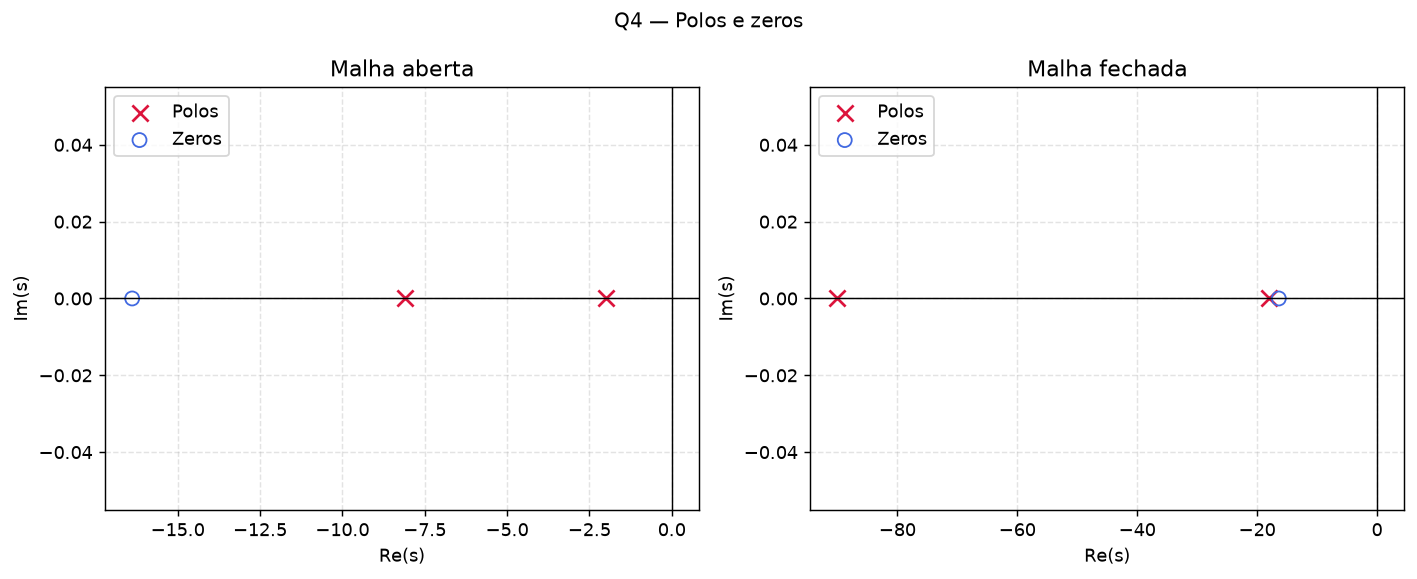
\includegraphics[width=\linewidth]{figuras/q4_polos.png}
    \caption{Polos e zeros}
  \end{subfigure}\hfill
  \begin{subfigure}[t]{0.48\linewidth}
    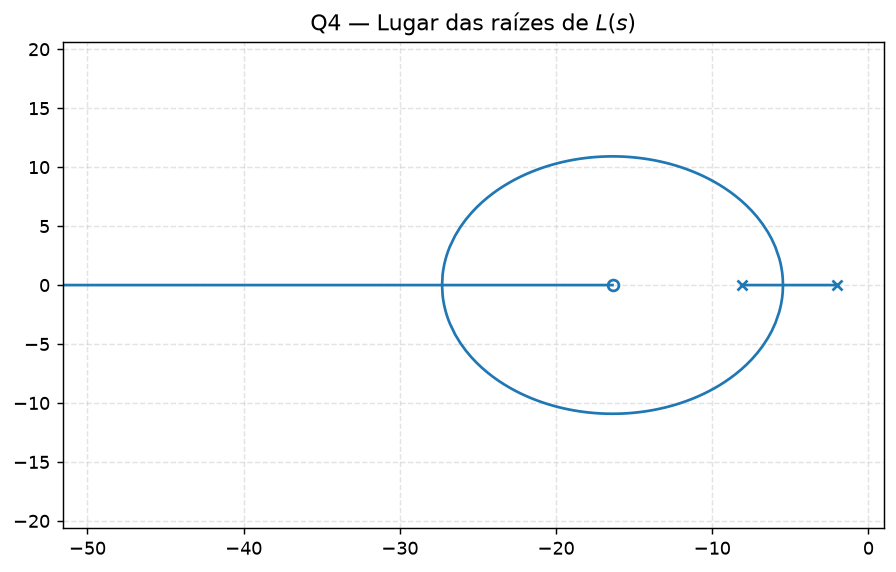
\includegraphics[width=\linewidth]{figuras/q4_lgr.png}
    \caption{Lugar das raízes}
  \end{subfigure}
  \caption{Questão~4 --- Plano-$s$ e LGR.}
\end{figure}

\textbf{Polos e LGR:} todos os polos são reais; o compensador molda a dinâmica
sem integrador (malha tipo~0). Leve sobressinal ($\approx 4\%$) decorre do zero
em $s\approx -16{,}4$, próximo ao polo dominante.

\begin{figure}[H]
  \centering
  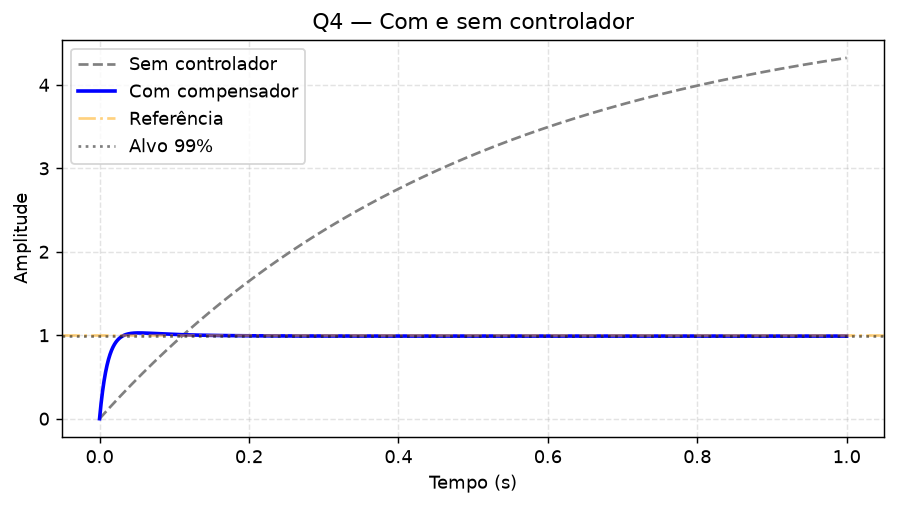
\includegraphics[width=0.75\linewidth]{figuras/q4_comparacao.png}
  \caption{Questão~4 --- Com e sem compensador.}
\end{figure}

\textbf{Comparação:} sem controlador, o ganho DC é $\approx 0{,}83$ (erro de
25\%); com o compensador, o sistema atinge 99\% do valor de referência.

%==============================================================================
\section*{Questão 5}
%==============================================================================

\textbf{Planta:} $G(s)=\dfrac{4}{(s+1)(s+3)(s+4)}$. \textbf{Requisitos:} erro
nulo; $\zeta=0{,}7$; $T_s=1{,}5\,\mathrm{s}$ (5\%).

\textbf{Controlador PID:}
$C(s)=\dfrac{2{,}04s^2+8{,}16s+6{,}12}{s}$.

\subsection*{Gráficos e análise}

\begin{figure}[H]
  \centering
  \begin{subfigure}[t]{0.48\linewidth}
    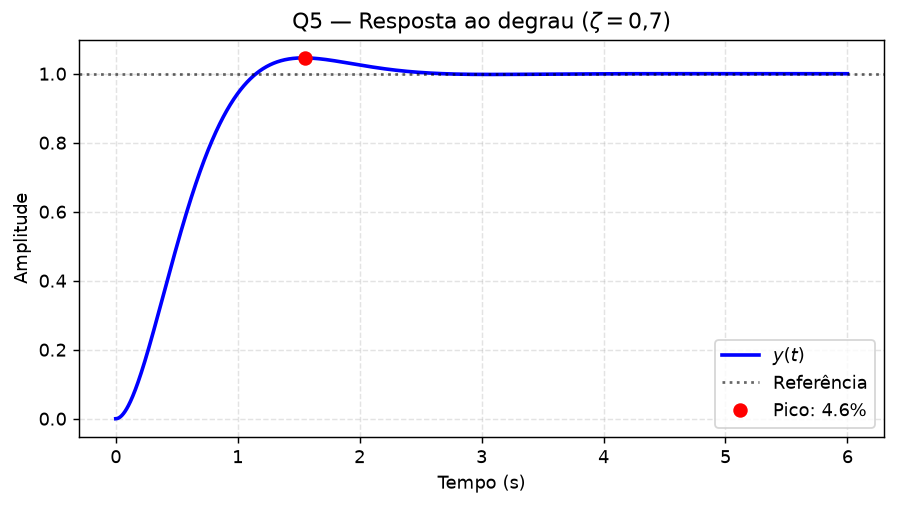
\includegraphics[width=\linewidth]{figuras/q5_degrau.png}
    \caption{Resposta ao degrau}
  \end{subfigure}\hfill
  \begin{subfigure}[t]{0.48\linewidth}
    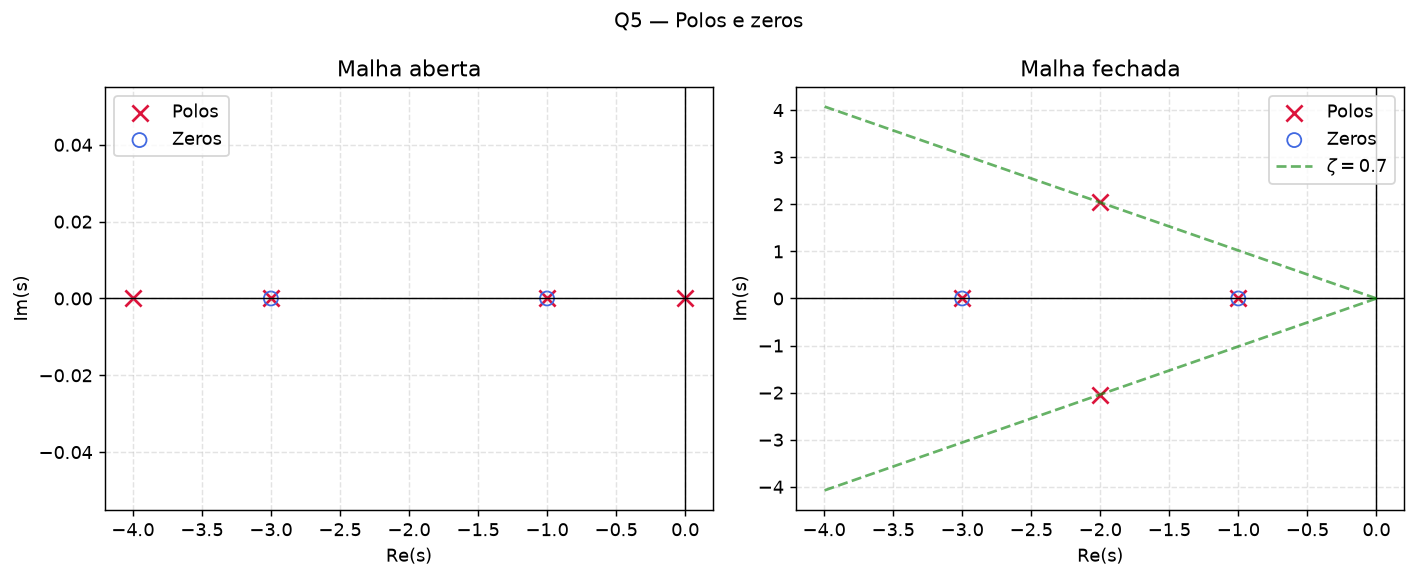
\includegraphics[width=\linewidth]{figuras/q5_polos.png}
    \caption{Polos e zeros}
  \end{subfigure}
  \caption{Questão~5 --- Resposta transitória e plano-$s$.}
\end{figure}

\textbf{Resposta ao degrau:} subamortecida com $\zeta=0{,}7$ e $e_{ss}=0$.
O $T_s$ simulado ($\approx 2{,}1\,\mathrm{s}$) excede o valor de~1,5~s porque
o polo lento em $s=-1$, imposto pela estrutura da planta (coeficiente de $s^3$
fixo em~8), retarda a acomodação global.

\textbf{Polos e zeros:} par dominante em $s=-2\pm j2{,}04$; polos auxiliares
reais em $s=-1$ e $s=-3$.

\begin{figure}[H]
  \centering
  \begin{subfigure}[t]{0.48\linewidth}
    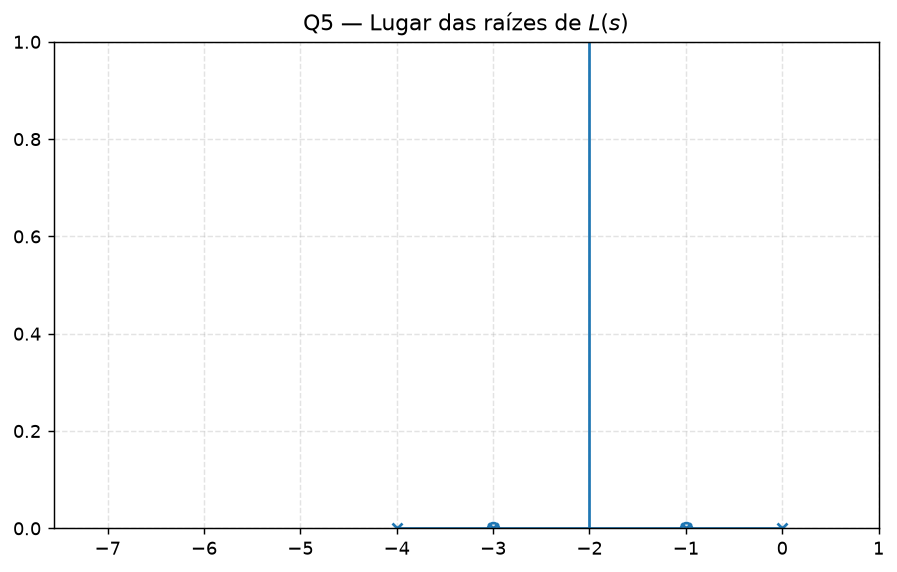
\includegraphics[width=\linewidth]{figuras/q5_lgr.png}
    \caption{Lugar das raízes}
  \end{subfigure}\hfill
  \begin{subfigure}[t]{0.48\linewidth}
    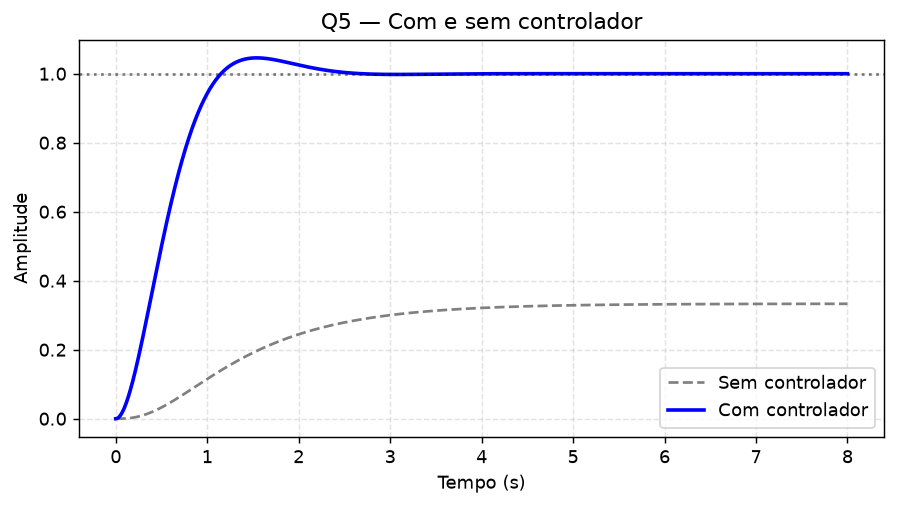
\includegraphics[width=\linewidth]{figuras/q5_comparacao.png}
    \caption{Com e sem controlador}
  \end{subfigure}
  \caption{Questão~5 --- LGR e comparação.}
\end{figure}

\textbf{LGR e comparação:} o PID elimina o erro estacionário de 75\% da planta
sem controlador e impõe o amortecimento desejado no par dominante.

%==============================================================================
\section*{Questão 6}
%==============================================================================

\textbf{Planta:} mesma da questão~5. \textbf{Método:} PI por Ziegler-Nichols em
malha fechada ($K_u=35$, $P_u\approx 1{,}44\,\mathrm{s}$).

\textbf{Controlador PI:}
$C(s)=15{,}75+\dfrac{13{,}11}{s}$.

\subsection*{Gráficos e análise}

\begin{figure}[H]
  \centering
  \begin{subfigure}[t]{0.48\linewidth}
    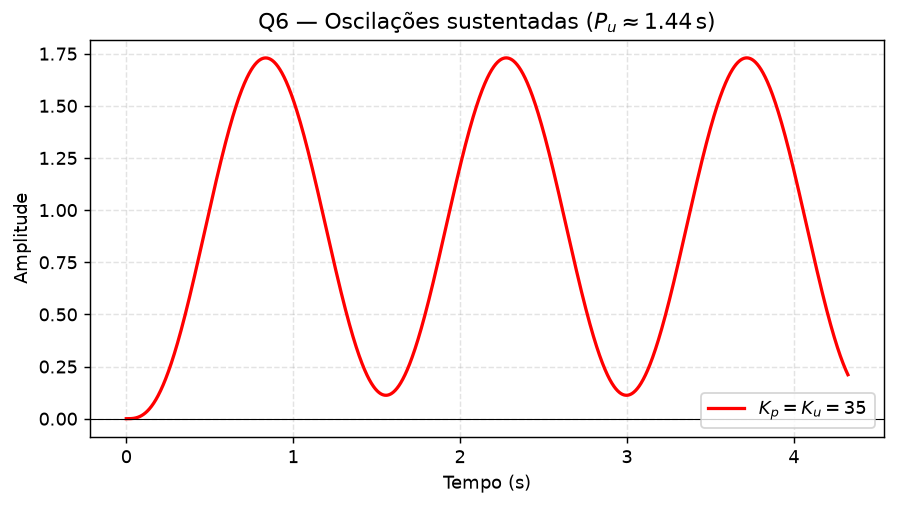
\includegraphics[width=\linewidth]{figuras/q6_critico.png}
    \caption{Oscilações em $K_u$}
  \end{subfigure}\hfill
  \begin{subfigure}[t]{0.48\linewidth}
    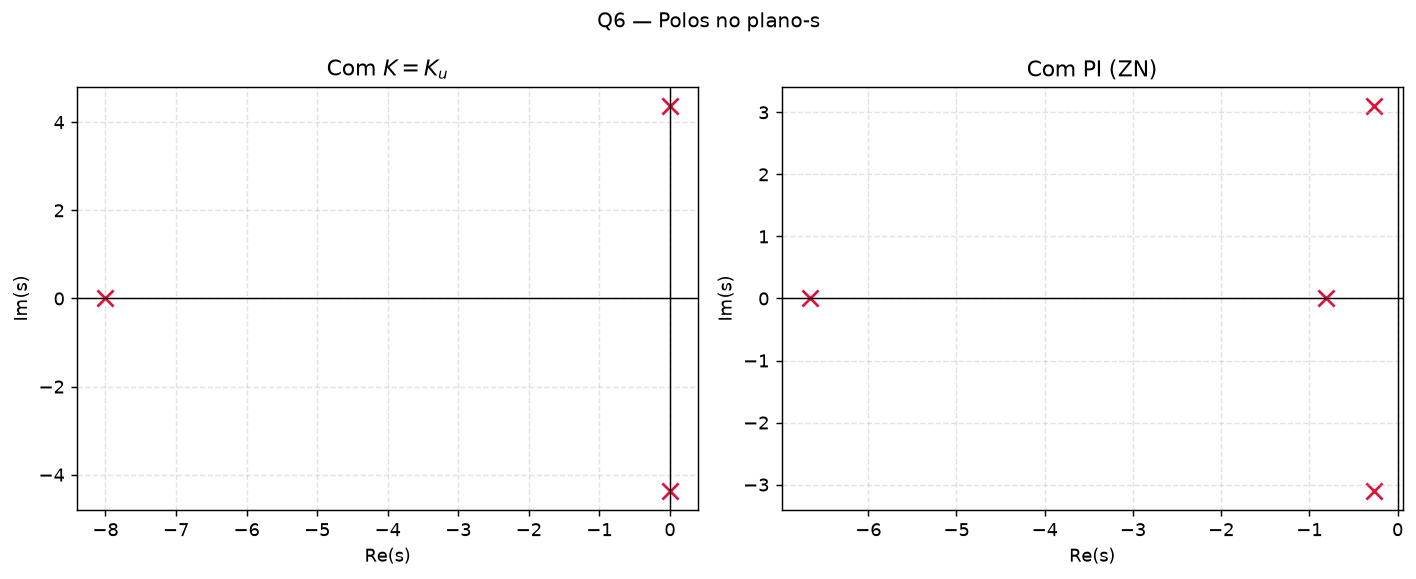
\includegraphics[width=\linewidth]{figuras/q6_polos.png}
    \caption{Polos: crítico vs.\ PI}
  \end{subfigure}
  \caption{Questão~6 --- Determinação de $K_u$ e $P_u$.}
\end{figure}

\textbf{Oscilações sustentadas:} com $K_p=K_u=35$, a resposta não se amortiza;
o período medido confirma $P_u\approx 1{,}44\,\mathrm{s}$. Os polos complexos
estão sobre o eixo imaginário em $s=\pm j\sqrt{19}$.

\textbf{Polos:} com o PI sintonizado, todos os polos migram para o semiplano
esquerdo, porém o par dominante permanece próximo do eixo imaginário.

\begin{figure}[H]
  \centering
  \begin{subfigure}[t]{0.48\linewidth}
    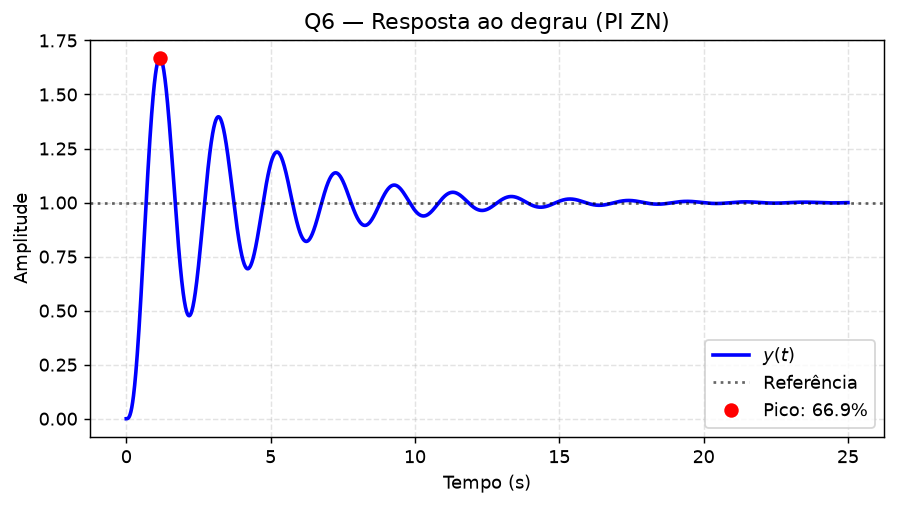
\includegraphics[width=\linewidth]{figuras/q6_degrau.png}
    \caption{Resposta PI (ZN)}
  \end{subfigure}\hfill
  \begin{subfigure}[t]{0.48\linewidth}
    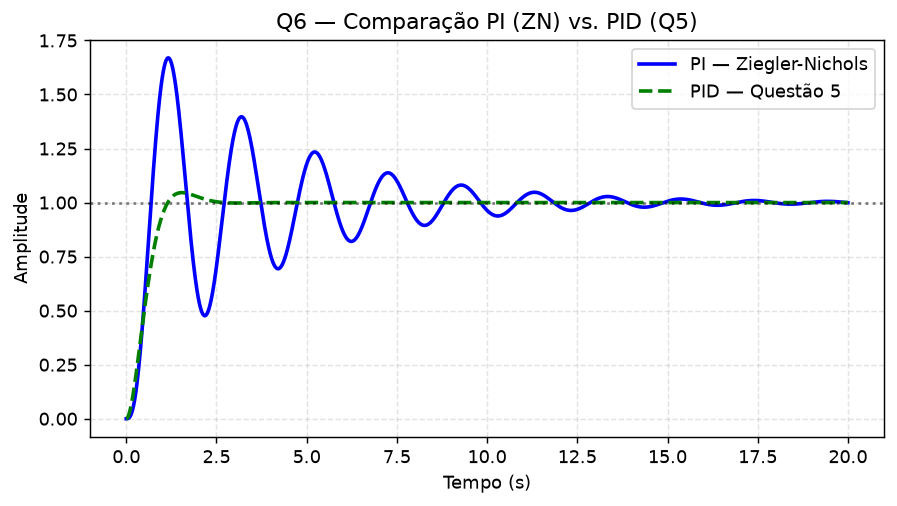
\includegraphics[width=\linewidth]{figuras/q6_comparacao.png}
    \caption{PI (ZN) vs.\ PID (Q5)}
  \end{subfigure}
  \caption{Questão~6 --- Desempenho do PI sintonizado.}
\end{figure}

\textbf{Resposta PI:} $e_{ss}=0$, porém sobressinal elevado ($\approx 67\%$) e
$T_s$ longo ($\approx 14{,}5\,\mathrm{s}$), típico do ZN.

\textbf{Comparação com Q5:} o PID analítico oferece resposta muito mais rápida
e amortecida; o ZN é mais simples de sintonizar, porém menos preciso em
requisitos transitórios.

%==============================================================================
\section*{Questão 7}
%==============================================================================

\textbf{Planta:} $G(s)=\dfrac{400}{s(s+40)}$. \textbf{Requisitos:}
$M_p\approx 20\%$; $T_s=1{,}5\,\mathrm{s}$ (2\%).

\textbf{Controlador PI ajustado:}
$C(s)=0{,}53+\dfrac{1{,}05}{s}$.

\subsection*{Gráficos e análise}

\begin{figure}[H]
  \centering
  \begin{subfigure}[t]{0.48\linewidth}
    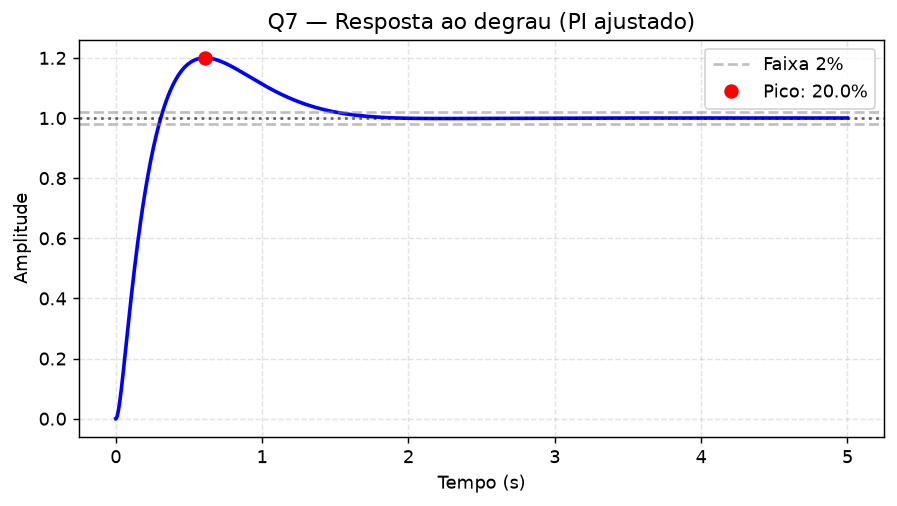
\includegraphics[width=\linewidth]{figuras/q7_degrau.png}
    \caption{Resposta ao degrau}
  \end{subfigure}\hfill
  \begin{subfigure}[t]{0.48\linewidth}
    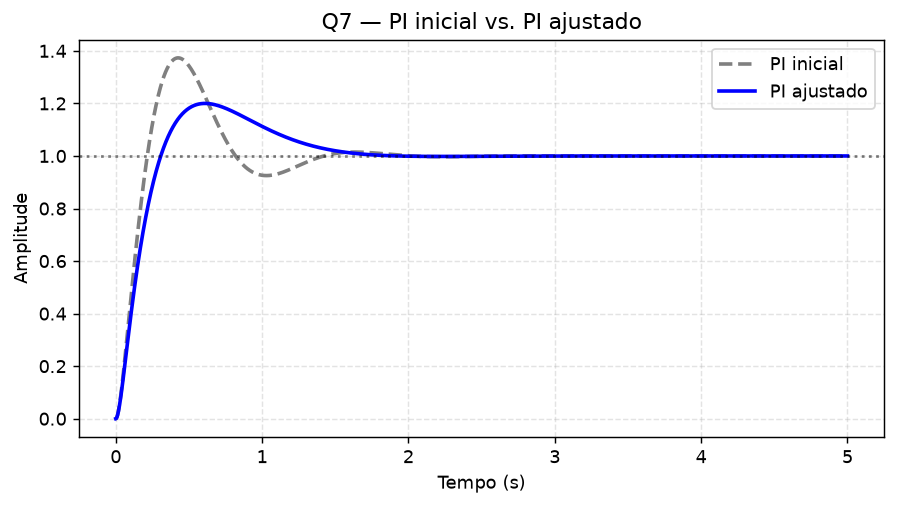
\includegraphics[width=\linewidth]{figuras/q7_ajuste.png}
    \caption{PI inicial vs.\ ajustado}
  \end{subfigure}
  \caption{Questão~7 --- Resposta e ajuste de ganhos.}
\end{figure}

\textbf{Resposta ao degrau:} sobressinal de \textbf{20,0\%} e
$T_s=\textbf{1,50}\,\mathrm{s}$, atendendo as especificações. Faixas de 2\%
destacadas no gráfico.

\textbf{Ajuste de ganhos:} a colocação direta ($K_p=0{,}55$, $K_i=2{,}97$)
produz sobressinal de $\approx 37\%$; o zero do PI e a malha tipo~2 alteram a
resposta. O ajuste para $K_p=0{,}53$, $K_i=1{,}05$ corrige $M_p$ e $T_s$.

\begin{figure}[H]
  \centering
  \begin{subfigure}[t]{0.48\linewidth}
    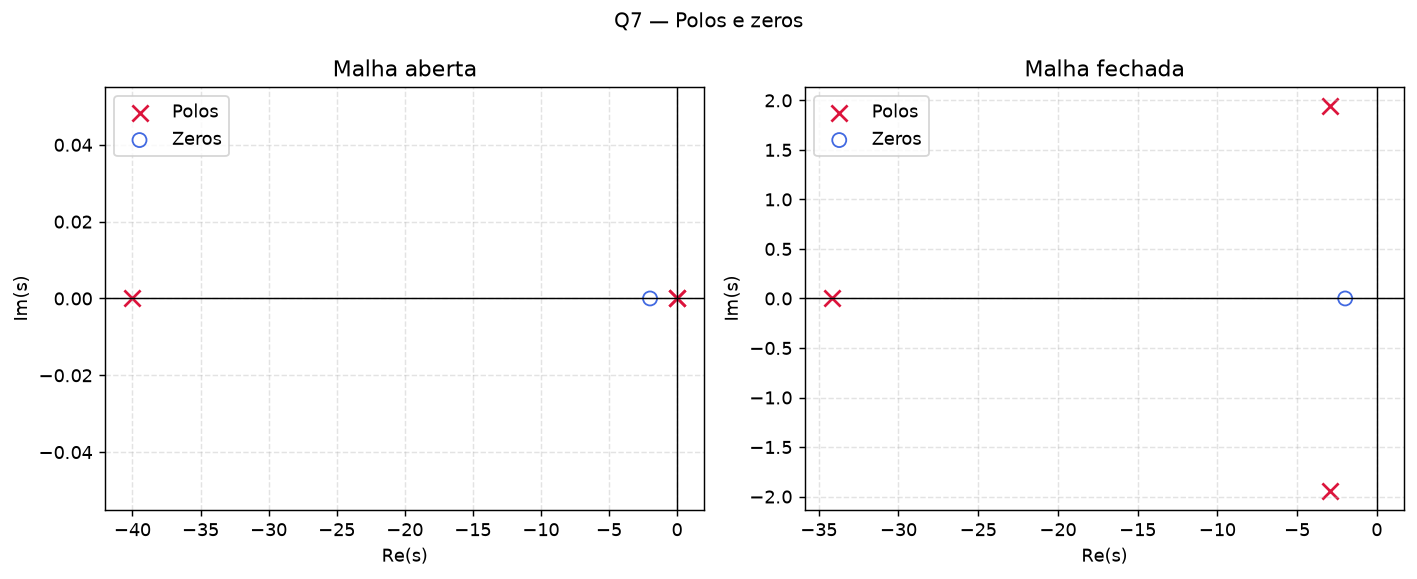
\includegraphics[width=\linewidth]{figuras/q7_polos.png}
    \caption{Polos e zeros}
  \end{subfigure}\hfill
  \begin{subfigure}[t]{0.48\linewidth}
    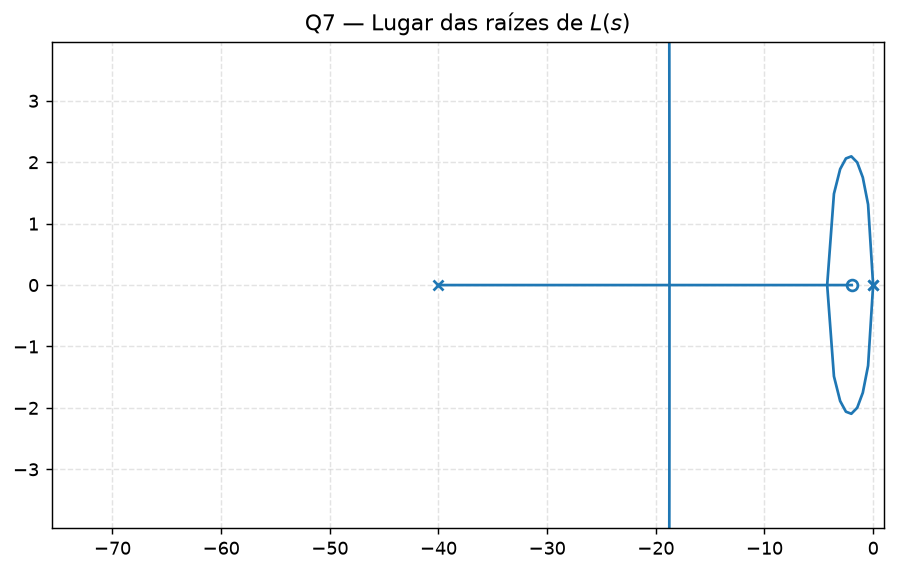
\includegraphics[width=\linewidth]{figuras/q7_lgr.png}
    \caption{Lugar das raízes}
  \end{subfigure}
  \caption{Questão~7 --- Plano-$s$ e LGR.}
\end{figure}

\textbf{Polos:} par dominante em $s\approx -2{,}92\pm j1{,}94$; polo rápido em
$s\approx -34{,}2$; zero do PI em $s\approx -1{,}98$ influencia o sobressinal.

\begin{figure}[H]
  \centering
  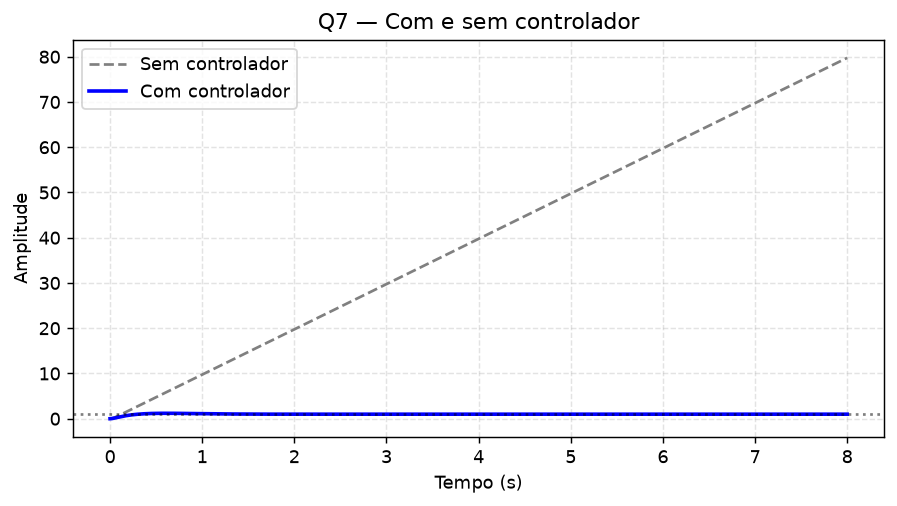
\includegraphics[width=0.75\linewidth]{figuras/q7_comparacao.png}
  \caption{Questão~7 --- Com e sem controlador.}
\end{figure}

\textbf{Comparação:} sem controlador, a resposta é lenta; com o PI ajustado, o
sistema atende $M_p$ e $T_s$ simultaneamente com $e_{ss}=0$.

%==============================================================================
\section*{Questão 8}
%==============================================================================

\textbf{Planta:} $G(s)=\dfrac{3}{(5s+1)(6s+1)}$. \textbf{Requisitos:} erro
nulo; $\zeta=0{,}43$.

\textbf{Controlador PID:}
$C(s)=\dfrac{104{,}93s^2+95{,}67s+100}{s}$.

\subsection*{Gráficos e análise}

\begin{figure}[H]
  \centering
  \begin{subfigure}[t]{0.48\linewidth}
    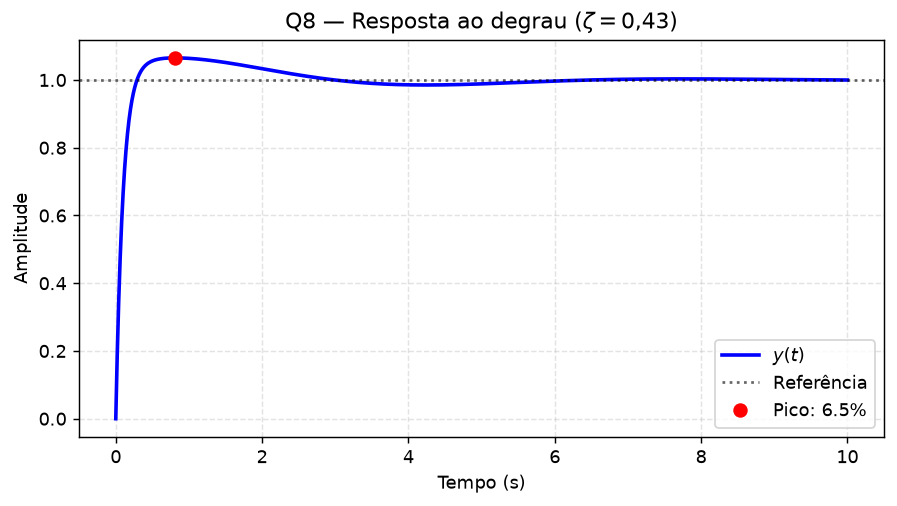
\includegraphics[width=\linewidth]{figuras/q8_degrau.png}
    \caption{Resposta ao degrau}
  \end{subfigure}\hfill
  \begin{subfigure}[t]{0.48\linewidth}
    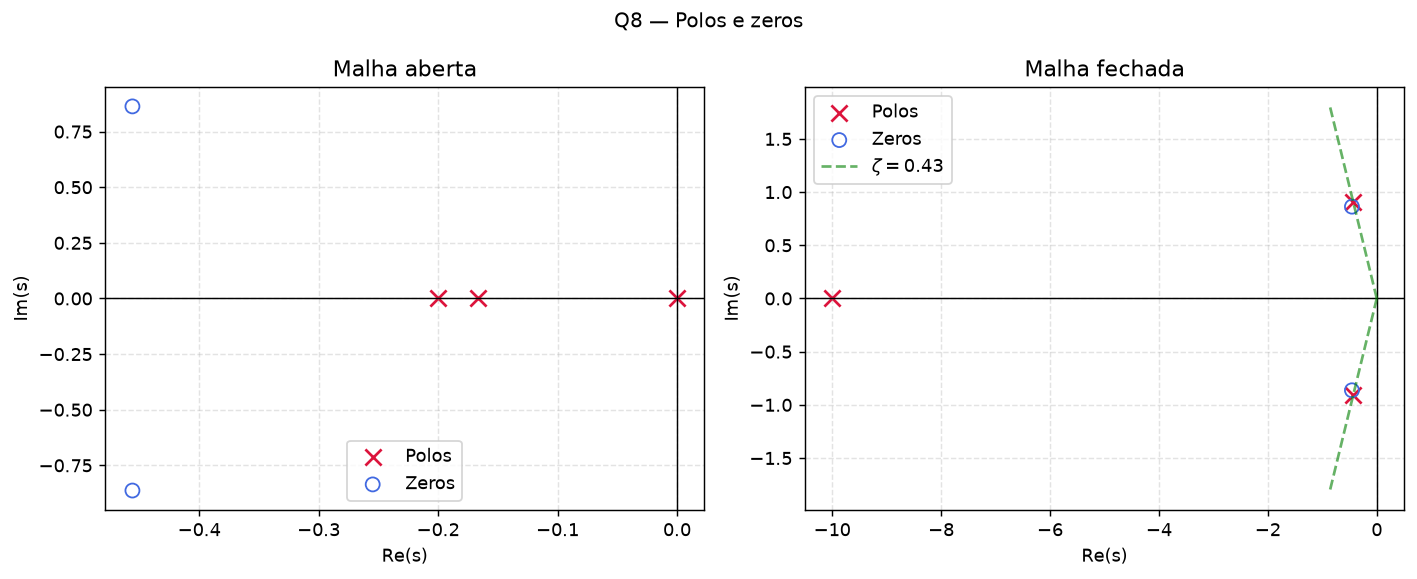
\includegraphics[width=\linewidth]{figuras/q8_polos.png}
    \caption{Polos e zeros}
  \end{subfigure}
  \caption{Questão~8 --- Resposta transitória e plano-$s$.}
\end{figure}

\textbf{Resposta ao degrau:} subamortecida com $\zeta=0{,}43$ e sobressinal
$\approx 6{,}5\%$ (menor que o teórico de 2ª ordem pura, devido aos zeros da
malha fechada). $e_{ss}=0$.

\textbf{Polos e zeros:} par dominante em $s=-0{,}43\pm j0{,}90$; polo real em
$s=-10$ não interfere no transitório.

\begin{figure}[H]
  \centering
  \begin{subfigure}[t]{0.48\linewidth}
    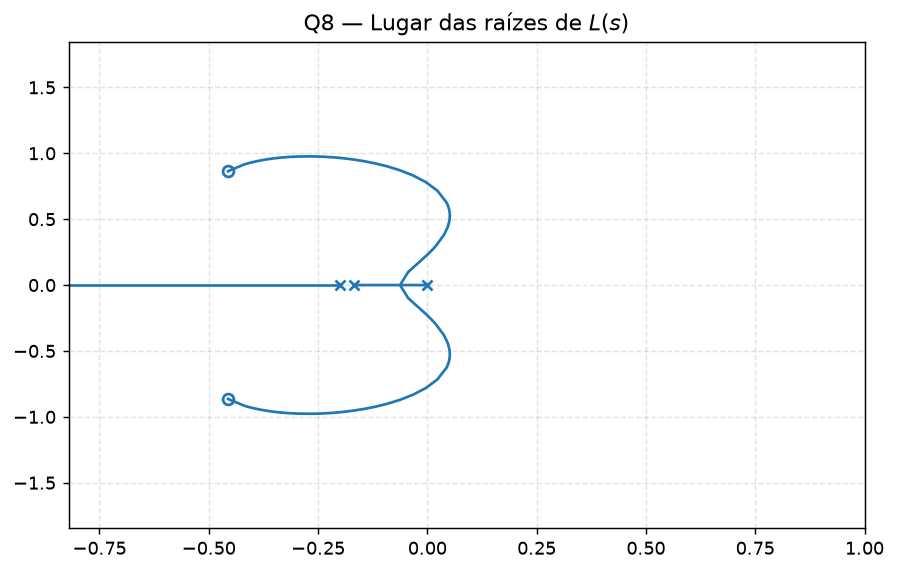
\includegraphics[width=\linewidth]{figuras/q8_lgr.png}
    \caption{Lugar das raízes}
  \end{subfigure}\hfill
  \begin{subfigure}[t]{0.48\linewidth}
    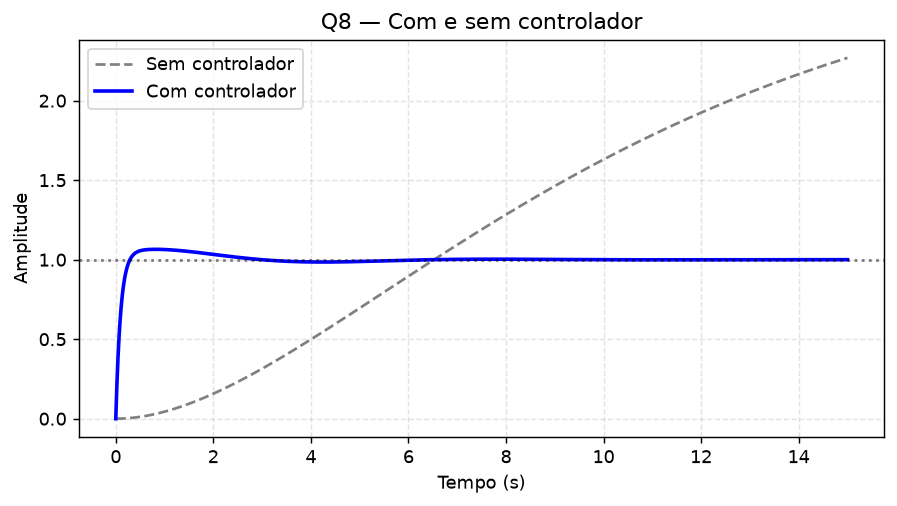
\includegraphics[width=\linewidth]{figuras/q8_comparacao.png}
    \caption{Com e sem controlador}
  \end{subfigure}
  \caption{Questão~8 --- LGR e comparação.}
\end{figure}

\textbf{LGR e comparação:} o PID desloca os ramos para a região com
$\zeta=0{,}43$ e elimina o erro estacionário de 25\% da planta sem
compensação.

%==============================================================================
\section*{Verificação geral}
%==============================================================================

\begin{table}[H]
  \centering
  \caption{Resumo do atendimento às especificações.}
  \label{tab:resumo}
  \begin{tabular}{@{}clccc@{}}
    \toprule
    Q & Controlador & $e_{ss}$ & $\zeta$ / tipo & $T_s$ ou $M_p$ \\
    \midrule
    1 & PID & $0$ & Sobreamort. & $\approx 1{,}2\,\mathrm{s}$ \\
    2 & PID & $0$ & $0{,}70$ & --- \\
    3 & PD  & $0$ & $0{,}50$ & $\approx 0{,}3\,\mathrm{s}$ \\
    4 & Atraso & $1\%$ & Sobreamort. & $\approx 0{,}1\,\mathrm{s}$ \\
    5 & PID & $0$ & $0{,}70$ & $\approx 2{,}1\,\mathrm{s}$$^{*}$ \\
    6 & PI (ZN) & $0$ & --- & --- \\
    7 & PI  & $0$ & --- & $M_p=20\%$, $T_s=1{,}5\,\mathrm{s}$ \\
    8 & PID & $0$ & $0{,}43$ & --- \\
    \bottomrule
  \end{tabular}
  \\[4pt]
  {\small $^{*}$Par dominante satisfaz $T_s=1{,}5\,\mathrm{s}$; resposta global
  mais lenta (polo em $s=-1$).}
\end{table}

\end{document}
